\documentclass[fr]{../../../eplsummary}
\usepackage{multirow}
\usepackage{../../../eplunits}
\usepackage{centernot}

\hypertitle{Mod\`eles et m\'ethodes d'optimisation}{4}{INMA}{1702}
{Beno\^it Legat \and Gilles Peiffer}
{François Glineur}

\newcommand{\libre}{\ensuremath{\textnormal{ libre}}}
\newcommand{\redcost}{\tilde{c}} % Coût réduits
\newcommand{\xopt}{\ensuremath{x^*}}
\newcommand{\adset}{\mathcal{D}}
\newcommand{\eqset}{\mathcal{E}}
\newcommand{\inset}{\mathcal{I}}
\newcommand{\acset}{\mathcal{A}}
\newcommand{\lagr}{\mathcal{L}}
\newcommand{\dset}{\mathcal{C}}
\newcommand{\polye}{\mathcal{P}}
\newcommand{\sign}{\mathrm{sign}}
\newcommand{\rpm}{\sbox0{$1$}\sbox2{$\scriptstyle\pm$}
  \raise\dimexpr(\ht0-\ht2)/2\relax\box2 }
\newcommand*\mean[1]{\bar{#1}}

\part{Convexité}
\section{Convexité d'une fonction}
\begin{mydef}[Convexité et concavité d'une fonction]
  Une fonction $f: \Rn \to \R$ est \emph{convexe} si et seulement si
  $\forall x, y \in \Rn$,
  \begin{align*}
    f(\lambda x + (1-\lambda)y) & \leq
    \lambda f(x) + (1-\lambda)f(y) & 0 \leq \lambda \leq 1.
  \end{align*}
  $f$ est concave si et seulement si $-f$ est convexe.
\end{mydef}

\begin{myprop}
  Soient $f_i: \Rn \to \R$ des fonctions convexes.
  Si on définit $f$ par
  \[ f(x) = \max_i f_i(x) \]
  alors $f$ est convexe.
\end{myprop}
\begin{myprop}
  Soit $f: \Rn \to \R$ défini par
  \[ f(x) = \max_{1 \leq i \leq k}(c_i^Tx + b_i), \]
  $f$ est convexe.
  On dit que $f$ est linéaire par morceaux.
\end{myprop}

\begin{myprop}
  Si $f:\adset\to\R$ est une fonction deux fois différentiable
  avec $\adset$ \emph{ouvert},
  $f$ est convexe si et seulement si $\adset$ est \emph{convexe} et
  \begin{align*}
    \grad^* f(x) & \succeq 0 & \forall x \in \adset.
  \end{align*}
\end{myprop}

\begin{myprop}
  Les fonctions \emph{affines} sont les seules fonctions qui sont à la fois
  concaves et convexes.
\end{myprop}

\section{Convexité d'un ensemble}
\begin{mydef}
  Soit un ensemble $\Omega \subseteq \Rn$.
  $\Omega$ est convexe si et seulement si, $\forall x, y \in \Omega$,
  \begin{align*}
    \lambda x + (1-\lambda) y & \in \Omega & 0 \leq \lambda \leq 1
  \end{align*}
\end{mydef}
\begin{myprop}
  \label{prop:interconv}
  Si $\Omega_1$ et $\Omega_2$ sont deux ensembles convexes,
  $\Omega_1 \cap \Omega_2$ est convexe.
\end{myprop}
\begin{myprop}
  Un demi-espace est convexe.
  La propriété~\ref{prop:interconv} nous permet alors de dire que
  tout hyperplan et tout polyèdre est convexe également car c'est
  l'intersection de demi-espaces.
\end{myprop}
\begin{myprop}
  Pour une fonction convexe, tout minimum local est un minimum global.
  L'ensemble des minima est convexe.
\end{myprop}

\begin{myprop}
  Si
  \[ \Omega = \{x \in \Rn \suchthat c_i(x) = 0\,\forall i \in \eqset
  \land c_i(x) \geq 0\,\forall i \in \inset\}, \]
  on a une condition \emph{suffisante} permettant de savoir si $\Omega$ est
  convexe.
  $\Omega$ est convexe si
  \begin{itemize}
    \item $c_i$ est \emph{affine} $\forall i \in \eqset$;
    \item $c_i$ est \emph{concave} $\forall i \in \inset$.
  \end{itemize}
\end{myprop}

\subsection{Convexité d'un problème}
\begin{mydef}[Convexité]
  Un problème de \emph{minimisation} est convexe si et seulement si
  $f$ est une \emph{fonction convexe} et
  $\adset$ est un \emph{ensemble convexe}.

  Un problème de \emph{maximisation} est convexe si et seulement si
  $f$ est une \emph{fonction concave} et
  $\adset$ est un \emph{ensemble convexe}.
\end{mydef}

\begin{myprop}
  \label{prop:loc2glob}
  Si un problème est convexe,
  tous les minima (resp. maxima) locaux sont globaux.
\end{myprop}
\begin{myprop}
  L'ensemble des minima (resp. maxima) forme un ensemble \emph{convexe}.
\end{myprop}

\part{Optimisation linéaire}
Il est important de préciser que lorsqu'on parle d'un vecteur,
celui-ci est nécessairement un \emph{vecteur colonne}.

\begin{mydef}[Opérateur de comparaison entre non scalaires]
  Dans le cadre de ce cours, définissons les opérateurs de comparaison $>$ et $<$
  pour les vecteurs et matrices comme vrais si ils sont respectés composante
  par composante et faux sinon.
  Par exemple, $(1, 2) > (0, -1)$ mais ni $(1, 1) > (0, 2)$,
  ni $(1, 1) < (0, 2)$ ne sont vrais.
  Certains vecteurs peuvent donc être incomparables.
\end{mydef}

\begin{mydef}[Problème d'optimisation linéaire]
  Un problème d'optimisation linéaire est un problème de la forme
  \begin{align*}
    \min_{(\text{resp. }\max)} \sum c^T x\\
    \sum a_i^T x & \leq b_j & \forall &i \in M_1\\
    \sum a_i^T x & \geq b_j & \forall &i \in M_2\\
    \sum a_i^T x & = b_j & \forall &i \in M_3\\
    x_i & \geq 0 & \forall &i \in N_1\\
    x_i & \leq 0 & \forall &i \in N_2
  \end{align*}
  On appelle $f(x) = c^Tx$ la fonction objectif.
  Tout $x \in \Rn$ est appelé une solution et s'il respecte les contraintes
  on dit que c'est une solution admissible.
  L'ensemble admissible, noté $\adset$, est l'ensemble des solutions
  admissibles.
  Si en plus il minimise (resp. maximise) $f$ parmi les solutions admissibles,
  c'est une solution optimale.
  $f(x)$ est alors le coût optimal, qui est unique.
  Il peut y avoir par contre une infinité de solutions optimales.
  Le coût peut aussi être non borné.
\end{mydef}

\begin{myrem}
  Les inégalités ne peuvent pas être strictes (pas par exemple $x > 0$).
\end{myrem}
\begin{myrem}
  L'ensemble des solutions admissibles est un polyèdre.
  La solution optimale se trouve sur un sommet de ce polyèdre si elle est unique, et sur une arête liant deux sommets si il y en a une infinité.
\end{myrem}

\section{Changement de forme}
On rappellera que pour une système de type
\[ Ax = b \]
on a
\begin{align*}
  A & = \begin{pmatrix}
  a_{11} & \cdots & a_{1n} \\
  \vdots & \ddots &  \vdots\\
  a_{m1} & \cdots & a_{mn}
  \end{pmatrix} &
  x & = \begin{pmatrix}x_1\\\vdots\\x_n\end{pmatrix} &
  b & = \begin{pmatrix}b_1\\\vdots\\b_m\end{pmatrix}. &
\end{align*}

Dans la matrice $A$, le vecteur $a_i$ est la $i$-ème ligne de $A$
et le vecteur $A_i$ la $i$-ème colonne.
On peut donc l'écrire de deux façons supplémentaires
\begin{align*}
  A & = \begin{pmatrix}a_1^T\\\vdots\\a_m^T\end{pmatrix} &
  A & = \begin{pmatrix}A_1 & \dots & A_n\end{pmatrix}.
\end{align*}

Tout problème d'optimisation peut toujours s'exprimer sous les deux
formes canoniques.
\begin{mydef}[Forme géométrique]
  \begin{align*}
    \min_x c^Tx\\
    Ax & \geq b.
  \end{align*}
\end{mydef}

$Ax \geq b$ devient alors $a_i^Tx \geq b_i$ pour $i = 1, \dots, m$.
En dimension $n$, $a_i^Tx = b_i$ définit un espace de dimension $n-1$.
L'inégalité nous impose d'être d'un côté de cet espace; ce qui définit
un demi-espace admissible.
L'intersection des $m$ demi-espaces donne l'espace admissible.

On peut montrer qu'on sait écrire n'importe quel
problème d'optimisation linéaire sous forme géométrique.

\begin{mydef}[Forme standard]
  \begin{align*}
    \min_x c^Tx\\
    Ax & = b\\
    x & \geq 0.
  \end{align*}
\end{mydef}
$Ax = b$ devient alors
\[ \sum_{i=1}^n A_ix_i = b. \]
Comme $x \geq 0$, l'ensemble des solutions admissible peut être interprété
par l'ensemble des coefficients de combinaisons linéaires positives des
colonnes de $A$ qui donne $b$.

Avec la forme géométrique, c'est plus facile de visualiser
mais avec la forme standard, c'est plus facile de résoudre.

\begin{myexem}
  Prenons le problème d'optimisation linéaire suivant
  \begin{align*}
    \max_x 2x_1 - x_2\\
    x_1 + x_2 & = 3\\
    2x_1 + x_2 & \leq 4\\
    9x_1 - x_2 & \geq 2\\
    x_2 & \leq 0
  \end{align*}
  Pour le transformer en forme géométrique,
  la transformation la plus astucieuse réside dans la transformation
  de $x_1 + x_3 = 3$ en $x_1 + x_3 \geq 3$ et en $x_1 + x_3 \leq 3$.
  On arrive donc à
  \begin{align*}
    -\min_x -2x_1 + x_2\\
    x_1 + x_2 & \geq 3\\
    -x_1 - x_2 & \geq -3\\
    -2x_1 - x_2 & \geq -4\\
    9x_1 - x_2 & \geq 2\\
    -x_2 & \geq 0.
  \end{align*}
\end{myexem}

Voyons maintenant si on peut transformer un problème sous forme géométrique
en problème sous forme standard.
Par transitivité, on pourra donc transformer n'importe quel
problème d'optimisation linéaire sous forme standard.
\begin{myexem}
  Prenons le problème d'optimisation linéaire suivant
  \begin{align*}
    \min_x 2x_1 + 4x_2\\
    x_1 + 3x_2 & \geq 3\\
    x_2 & \geq 0.
  \end{align*}
  Commençons par introduire une variable d'écart (\emph{slack variable})
  pour avoir une équation et non plus une inéquation
  \begin{align*}
    \min_x 2x_1 + 4x_2\\
    x_1 + 3x_2 - x_3 & = 3\\
    x_2 & \geq 0\\
    x_3 & \geq 0.
  \end{align*}
  Éliminons maintenant les variables libres qui sont ici $x_1$ en
  posant $x_1^+, x_1^- \geq 0$ tels que $x_1 = x_1^+ - x_1^-$
  \begin{align*}
    \min_x 2x_1^+ - 2x_1^- + 4x_2\\
    x_1^+ - x_1^- + 3x_2 - x_3 & = 3\\
    x_1^+, x_1^-, x_2, x_3 & \geq 0.
  \end{align*}
\end{myexem}

\begin{myprop}
  Soit $f(x)$ une fonction convexe linéaire par morceaux.
  \begin{align*}
    \min_x f(x)\\
    Ax \leq b
  \end{align*}
  peut être écrit sous la forme d'un problème d'optimisation linéaire.
\end{myprop}
\begin{myexem}
  \begin{align*}
    \min_{x_1,x_2} 2|x_1| + x_2\\
    x_1 + x_2 & \geq 4.
  \end{align*}
  On a
  \begin{align*}
    2 \abs{x_1}+x_2 & = \max(2x_1,-2x_1) + x_2\\
    & = \max(2x_1+x_2,-2x_1+x_2)\\
    & = \min\{t \suchthat t \geq 2x_1+x_2,t\geq -2x_1+x_2)\}.
  \end{align*}
  Le problème devient donc
  \begin{align*}
    \min_{x_1, x_2, t} t\\
    2x_1 + x_2 - t & \leq 0\\
    -2x_1 + x_2 - t & \leq 0\\
    x_1 + x_2 & \geq 4,
  \end{align*}
  qui est un problème d'optimisation linéaire.
\end{myexem}
\begin{myexem}
  \begin{align*}
    \min_{x} \max_i (c_i^Tx+b_i)\\
    Ax & \leq b
  \end{align*}
  est un problème d'optimisation linéaire.
  En effet, il peut être réécrit en
  \begin{align*}
    \min_{x,t} t\\
    c_i^Tx-t & \leq -b_i & i = 1, \dots, n\\
    Ax & \leq b.
  \end{align*}
\end{myexem}

\section{Géométrie des polyèdres}
\begin{mydef}[Hyperplan]
  Un hyperplan est défini par
  $\{ x \suchthat a^Tx=b \}$.
\end{mydef}
Le vecteur $a$ est un vecteur normal à l'hyperplan.
\begin{mydef}[Demi-espace]
  Un demi-espace est défini par
  $\{x \suchthat a^Tx\geq b\}$.
\end{mydef}
\begin{mydef}[Polyèdre]
  Un polyèdre est défini par
  \[ \{x \suchthat a_i^Tx \geq b_i, i = 1,\dots,m\}. \]
\end{mydef}
Un polyèdre borné est appelé un polytope.

\subsection{Sommets et contraintes serrées}
Soit $\polye$ le polyèdre défini par les contraintes
\begin{align*}
  a_i^T x & \geq b_i, & i \in M_1;\\
  a_i^T x & \leq b_i, & i \in M_2;\\
  a_i^T x & = b_i, & i \in M_3.
\end{align*}
Les contraintes sont dites linéairement indépendantes si les $a_i$ le sont.
Soit $\xopt \in \polye$,
la contrainte $i$ est dite \emph{serrée} ou \emph{active} si $a_i^T\xopt = b_i$.
Les contraintes $i \in M_3$ sont donc toujours serrées.

On peut caractériser un sommet par l'intersection de $n$ hyperplans
linéairement indépendants.
On va donc définir une solution admissible de base $\xopt$ comme une solution
telle qu'il y a $n$ contraintes linéairement indépendantes qui sont serrées.
S'il y a plus de $n$ contraintes actives (mais toujours que $n$ contraintes
actives linéairement indépendantes) on dit qu'elle est \emph{dégénérée}.

Deux solutions $x_1, x_2 \in \polye$ sont dites
\emph{adjacentes} s'il y a $n-1$ contraintes linéairement indépendantes qui sont
à la fois actives pour $x_1$ et $x_2$.

On peut aussi définir un \emph{point extrême} comme
un point qui ne peut être exprimé comme une combinaison convexe de deux
autres points du polyèdre.
C'est-à-dire que $x\in \polye$ est un point extrême s'il
n'existe pas $y,z \in \polye$ et
$0 \leq \lambda \leq 1$ tels que
\[ x = \lambda y + (1-\lambda)z. \]

Un \emph{sommet} est un point qui est séparable par un hyperplan.
C'est-à-dire que $x \in \polye$ est un sommet s'il existe $c$
tel que pour tout $y \in \polye\setminus\{x\}$,
\[ c^Tx < c^Ty. \]

Seulement, être un sommet, être un point extrême et être une solution
admissible de base sont 3 propositions équivalentes.

\subsubsection{Existence d'un sommet}
\begin{mydef}
  Un polyèdre $\polye$ contient une droite s'il existe un vecteur $x_0$
  et un vecteur non nul $d$ tels que $x_0 + \lambda d \in \polye$
  pour tout $\lambda \in \R$.
\end{mydef}

\begin{myprop}
  Un polyèdre possède un sommet si et seulement si il ne contient
  pas de droite.
\end{myprop}

\begin{myprop}
  Un polyèdre sous forme géométrique possède un sommet si et seulement si
  l'équation $Ad = 0$ n'a pas d'autre solution que $d = 0$.
\end{myprop}

\begin{myprop}
  Un polyèdre sous forme standard possède toujours un sommet.
\end{myprop}

\subsubsection{Sommet sous forme standard}
Supposons qu'on ait $n$ variables et $m$ contraintes d'égalité.
Supposons que les contraintes soient linéairement indépendantes.
Si $n \leq m$, on a au plus une solution admissible, c'est alors un sommet.
Sinon, les $m$ contraintes d'égalités ne suffisent pas pour faire un sommet.
Effectivement, en un sommet, on serre toujours autant de contraintes qu'il y a de variables.
On a donc besoin de $n-m$ contraintes serrées
en plus qu'on choisit dans $x \geq 0$.
Les variables qui n'ont pas ces contraintes serrées et qui sont donc
non nulles sont appellées les variables de base.
En réarrangeant les équations pour que ces variables apparaissent en premier,
on peut écrire
\begin{align*}
  \begin{pmatrix}
    B & N\\
    0 & I
  \end{pmatrix}
  \begin{pmatrix}
    x_B^*\\
    x_N^*
  \end{pmatrix} =
  \begin{pmatrix}
    b\\
    0
  \end{pmatrix}.
\end{align*}
Il faut néanmoins que les contraintes non serrées soient respectées,
c'est-à-dire que $x_B^* \geq 0$ ou encore $B^{-1}b \geq 0$ car
on voit bien que $x_B^* = B^{-1}b$.
Si une des composantes de $x_B^*$ est nulle on dit que c'est un
sommet dégénéré.

\section{Algorithme du simplexe}
\subsection{Théorème fondamental}
\begin{mytheo}[Théorème fondamental de l'optimisation linéaire]
  Sur un polyèdre, si
  \begin{enumerate}
    \item le polyèdre possède un sommet,
    \item le coût optimal est fini,
  \end{enumerate}
  alors il existe un sommet optimal.
\end{mytheo}
Une conséquence directe est que
\begin{mycorr}
  Si un polyèdre possède un sommet mais pas de sommet optimal, le coût optimal est infini.
\end{mycorr}
\begin{myrem}
  Il ne faut cependant pas faire dire au
  théorème fondamental ce qu'il ne dit pas.
  Si les conditions sont remplies, il \emph{existe} un sommet optimal mais
  toutes les solutions optimales ne sont pas nécessairement des sommets.
  Par exemple, pour le problème d'optimisation linéaire suivant
  \begin{align*}
    \min_{x_1} x_1\\
    (x_1,x_2) & \geq 0,
  \end{align*}
  la solution optimale $(0,0)$ est un sommet optimal mais la solution optimale $(0,1)$
  n'est pas un sommet.
\end{myrem}

\subsection{L'algorithme du simplexe}
L'algorithme du simplexe se base sur la forme standard.
On pose alors $z$ comme la variable à minimiser avec
\begin{align*}
  c^T x & = z\\
  Ax & = b\\
  x & \geq 0.
\end{align*}
On a donc $n$ variables,
$m$ contraintes dans $Ax = b$ et
$n$ contraintes dans $x \geq 0$.
Supposons que $m < n$ (sinon, à moins d'avoir des contraintes linéairements
dépendantes, l'ensemble admissible ne contient qu'un point ou est vide).
Pour avoir un sommet, il nous faut choisir
$m$ variables de base $x_B$ et $n-m$ variables hors base $x_N$.
\begin{align*}
  c_B^Tx_B + c_N^Tx_N & = z\\
  Bx_B + Nx_N & = b\\
  x_B,x_N & \geq 0.
\end{align*}
On transforme ensuite
\begin{align*}
  c_B^Tx_B + c_N^Tx_N & = z\\
  x_B + B^{-1}Nx_N & = B^{-1}b\\
  x_B, x_N & \geq 0
\end{align*}
\begin{align*}
  c_N^Tx_N-c_B^TB^{-1}Nx_N & = z - c_B^TB^{-1}b\\
  x_B + B^{-1}Nx_N & = B^{-1}b\\
  x_B, x_N & \geq 0.
\end{align*}
Le sommet
\begin{itemize}
  \item est admissible si et seulement si $B^{-1}b \geq 0$;
  \item est optimal si et seulement si
    \[ \tilde{c} = c_N^T - c_B^TB^{-1}N \geq 0. \]
    On appelle ça les \emph{coûts réduits};
  \item n'est pas dégénéré si et seulement si $x_B > 0$.
\end{itemize}
\begin{enumerate}
  \item Trouver une base $B$ et le sommet correspondant
    $(x_B = B^{-1}b \geq 0, x_N = 0)$.
  \item Calculer les coûts réduits $\redcost$:
    $\redcost^T = c_N^T - c_B^{T}B^{-1}N$.
    \begin{itemize}
      \item Si $\redcost \geq 0$, stop; $x$ est optimal;
      \item Sinon, on choisit un indice $j$ pour lequel $\redcost_j < 0$.
    \end{itemize}
  \item Calculer le vecteur $u = B^{-1}N_j$. % Where does this j come from...?
    \begin{itemize}
      \item Si $u \leq 0$, le coût optimal est non borné, stop.
    \end{itemize}
  \item Pour tous les $u_i > 0$, calculer $B_{i,i}/u_i$,
    soit $\lambda^*$ le minimum.
    On va choisir une ligne $l$ pour laquelle $B_{l,l}/u_l = \lambda^*$.
    La variable qui rentre dans la base est $x_j$ et la variable qui
    quitte la base est $x_l$.
  \item
    Calculer le tableau associé à la nouvelle base.
\end{enumerate}
On pourrait se dire que l'algorithme converge toujours
car le coût diminue toujours strictement.
On ne pourra donc pas faire de boucle et
comme il y a un nombre fini de sommets,
l'algorithme ne peut que converger.

Seulement, dans le cas de sommets dégénérés, il arrive qu'un pivotage
ne diminue pas $z$ mais ne le modifie pas.
En effet, ce qui diminue $z$, c'est quand,
lorsqu'on essaie de faire rentrer $x_j$ dans la base,
on met son coefficient dans la fonction objectif à 0.
Comme on avait un sommet admissible, le terme indépendant de l'équation
qu'on utilise était positif.

Et comme on avait choisi un $x_j$ qui a un coefficient négatif,
le terme indépendant de la fonction objectif augmente donc $z$ diminue.
Pour qu'il ne diminue pas,
il faut que le terme indépendant de l'équation soit nul, c'est-à-dire
qu'on ait $x_l = 0$ et donc un sommet dégénéré.

La convergence dépend donc de la stratégie adoptée dans le cas de sommets
dégénérés.
Il y a par exemple la règle de Bland qui dit qu'en cas d'égalité,
on prend toujours la variable avec le plus petit indice.

Il existe des cas pathologiques pour lesquels l'algorithme
du simplexe a une complexité exponentielle
mais en pratique, il est efficace.

Il existe aussi des méthodes du \emph{point intérieur},
dont l'algorithme de Karmarkar, introduit en 1984, qui garde une complexité polynomiale même dans
le pire des cas ($\bigoh(n^{3.5} L^2 \log L \log \log L)$ où $n$ est le nombre de variables et $L$ est le nombre de bits d'entrée de l'algorithme). % Crazy stuff :o

\begin{myexem}
  \label{ex:simplex}
  Rajoutons $z$
  \begin{align*}
    \min_z z\\
    x_2 - 5x_3+ 6x_4 & = z\\
    x_1 + x_2 - 11x_3 + 7x_4 & = 10\\
    x_2 - 8x_3 + 4x_4 & = 4\\
    x_i & \geq 0
  \end{align*}
  Tableau simplexe :
  \[
    \begin{array}{cccc|c}
      0 & 1 & -5 & 6 & z\\
      \hline
      1 & 1 & -11 & 7 & 10\\
      0 & 1 & -8 & 4 & 4
    \end{array}
  \]
  L'idée est d'arriver à la forme canonique du tableau simplexe.

  C'est-à-dire que pour $m$ variables de base, on doit avoir
  des $0$ dans la fonction objectif et la matrice identité
  dans la matrice des contraintes.
  Prenons comme base $\{x_1, x_2\}$ et
  donc comme variables hors base $\{x_3, x_4\}$.
  En utilisant des opérations élémentaires sur les lignes,
  essayons donc d'avoir
  \[
    \begin{array}{cccc|c}
      0 & 0 & ? & ? & ?\\
      \hline
      1 & 0 & ? & ? & ?\\
      0 & 1 & ? & ? & ?
    \end{array}
  \]
  Dans notre cas, ça donne
  \[
    \begin{array}{cccc|c}
      0 & 0 & 3 & 2 & z-4\\
      \hline
      1 & 0 & -3 & 3 & 6\\
      0 & 1 & -8 & 4 & 4
    \end{array}
  \]
  La manière de décrire la fonction objectif a changé
  mais la valeur prise lorsqu'on
  est dans le polyèdre est restée rigoureusement identique.
  3 et 2 sont les \emph{coûts réduits} de $x_3$ et $x_4$.

  On voit que $(6, 4, 0, 0)$ est un sommet car il serre aussi $x_3 = 0$
  et $x_4 = 0$.
  Comme la fonction objectif est
  $4 + 3x_3 + 2x_4 = z$, et que $x_3, x_4 \geq 0$, ce sommet est clairement
  optimal car 3 et 2 sont positifs.

  Si on avait eu
  \[
    \begin{array}{cccc|c}
      0 & 0 & -3 & 2 & z-4\\
      \hline
      1 & 0 & -3 & 3 & 6\\
      0 & 1 & -8 & 4 & 4
    \end{array}
  \]
  on aurait eu un coût réduit négatif et donc un coût optimal non borné.
  En effet, en prenant
  $x_4 = 0$ et $x_3 = \lambda > 0$, on a
  $x = (6 + 3\lambda, 4+8\lambda, \lambda, 0)$.
  Pour $\lambda \to +\infty$, toutes les contraintes sont respectées et
  $z \to -\infty$.

  Si on avait eu
  \[
    \begin{array}{cccc|c}
      0 & 0 & -3 & -2 & z-4\\
      \hline
      1 & 0 & 3 & 3 & 6\\
      0 & 1 & 6 & 4 & 4
    \end{array}
  \]
  on n'aurait rien pu conclure.
  On aurait donc dû voyager vers un sommet adjacent.
  Pour cela, il faut choisir une variable à faire rentrer dans la base.
  Disons $x_3$.
  Par contre, on ne peut pas faire sortir n'importe quelle variable
  de la base.
  Si on fait sortir la mauvaise, on risque d'avoir une solution non admissible.
  Pour savoir laquelle sortir, on pose $x_3 = \lambda$ et $x_4 = 0$.
  Les contraintes deviennent
  \begin{align*}
    x_1 + 3\lambda & = 6\\
    x_2 + 6\lambda & = 4
  \end{align*}
  Si on enlève $x_i$ de la base, on a $x_i = 0$.
  En retirant $x_1$, on a donc $\lambda = 2$ et en retirant $x_2$,
  on aura $\lambda = 2/3$.
  Déjà, on rejette celles où $\lambda < 0$.
  Ensuite, il faut prendre celle où $\lambda$ est le plus petit.
  En effet, si on avait retiré $x_1$, on aurait eu $\lambda = 2$
  et $x_2$ aurait donc du être négatif.
\end{myexem}

Comme on a vu dans l'exemple~\ref{ex:simplex},
si pour une variable hors base,
on a dans la fonction objectif un coefficient négatif et une colonne $\leq 0$
en dessous, le coût est non borné.


\subsection{Calcul d'un premier sommet}
Pour faire la méthode du simplexe,
il faut un premier sommet pour démarrer.
Pour calculer ce premier sommet,
on peut utiliser le problème annexe
\begin{align*}
  \min_y \sum_i y_i&\\
  Ax + y & = b\\
  x,y &\geq 0.
\end{align*}
On remarque que
pour que $x$ soit une solution admissible du problème de départ,
il faut qu'il existe une solution admissible avec $y=0$ pour le problème
annexe.
S'il existe une telle solution, la fonction objectif sera minimale et
vaudra 0.
Il suffit donc d'appliquer l'algorithme du simplexe sur le problème annexe.
Si le coût optimal est positif, c'est que l'ensemble admissible du
problème de départ est vide.
Sinon, le coût optimal est nul et le sommet optimal est $(\xopt,0)$
où $\xopt$ est une solution admissible du problème de départ.

Pour le problème annexe, le sommet de départ est très facile à obtenir;
c'est $(x,y) = (0,b)$.

\section{Dualité}
Tout problème d'optimisation linéaire a un problème \emph{dual}.
Le dual du dual est le problème de départ qu'on appelle le \emph{primal}.
Les variables du dual sont associées aux contraintes du primal.

La dualisation peut-être illustrée par la recherche d'une borne inférieure.
Le minimum devient donc la borne inférieure maximale qu'on sait
obtenir en faisant une combinaison linéaire des contraintes.

Pour trouver une borne valide, il faut faire une combinaison linéaire
telle que,
\begin{itemize}
  \item si $x_i$ est libre, le coefficient pour $x_i$ est égal à $c_i$;
  \item si $x_i \geq 0$, le coefficient pour $x_i$ est plus petit que $c_i$;
  \item si $x_i \leq 0$, le coefficient pour $x_i$ est plus grand que $c_i$.
\end{itemize}
En effet, si $x_i \leq 0$ et que le coefficient est plus grand que $c_i$,
on va être plus petit que la fonction objectif donc la borne restera valide.

Comme on fait une borne inférieure, il faut que les inégalités soient $\leq$.
Donc
\begin{itemize}
  \item si on a $a_i^Tx = b_i$, $y_i$ est libre;
  \item si on a $a_i^Tx \geq b_i$, $y_i \geq 0$ pour garder
    le sens de l'inégalité;
  \item si on a $a_i^Tx \leq b_i$, $y_i \leq 0$ pour renverser
    le sens de l'inégalité.
\end{itemize}

\begin{mytheo}[Dualité d'un problème sous forme générale]
  \begin{align*}
    \min_x c^T x & & \max_y b^Ty\\
    a_i^Tx & = b_i & y_i & \libre\\
    a_i^Tx & \geq b_i & y_i & \geq 0\\
    a_i^Tx & \leq b_i & y_i & \leq 0\\
    x_j & \libre & A_j^T y & = c_j\\
    x_j & \geq 0 & A_j^Ty & \leq c_j\\
    x_j & \leq 0 & A_j^Ty & \geq c_j\\
    \textnormal{Primal} & & \textnormal{Dual}
  \end{align*}
\end{mytheo}
\begin{mytheo}[Dualité sous forme géométrique]
  \begin{align*}
    \min_x c^Tx & & \max_y b^Ty\\
    Ax & \geq b & y_i & \geq 0\\
    & & A^Ty & = c
  \end{align*}
\end{mytheo}

\begin{mytheo}[Dualité sous forme standard]
  \begin{align*}
    \min_x c^Tx & & \max_y b^Ty\\
    Ax & = b & A^Ty & \leq c\\
    x & \geq 0 & y & \libre
  \end{align*}
  La solution optimale du dual est donnée par $(y^*)^T = c_B^TB^{-1}$.
  Pour rappel, $x_B = B^{-1}b$.
\end{mytheo}

\begin{myprop}[Dualité faible]
  Si $Ax \geq b$ et $x \geq 0$. $A^Ty \leq c$ et $y \geq 0$.
  Alors $c^Tx \geq b^Ty$.
  En particulier $z^* = \min_x c^T x \geq \max_y b^Ty = w^*$.
  $c^Tx-b^Ty$ est l'\emph{écart dual}.
  \begin{proof}
    En effet,
    \[ c^Tx \geq y^TAx \geq b^Ty. \]
  \end{proof}
\end{myprop}

\begin{mycorr}
  Si $x$ est une solution admissible du dual et $y$ la solution
  admissible du primal correspondante
  et que $c^Tx = b^Ty$, alors $x$ et $y$ sont
  des solutions optimales de leurs problèmes respectifs.
\end{mycorr}

\begin{mytheo}[Dualité forte]
  Si un des problèmes possède une solution optimale alors l'autre en possède
  également et les objectifs optimaux sont égaux.
  \begin{proof}
    Dans un cas particulier.
    \begin{align*}
      \min_x c^T x & & \max_y b^T y\\
      Ax & = b & A^Ty & \leq c\\
      x & \geq 0
    \end{align*}
    Posons $\xopt$ optimal.
    On a que $\xopt = (x_B, x_N)$. On sait également que
    $x_N = 0$, $x_B = B^{-1}b \geq 0$ et $c_N^T - c_B^T N \geq 0$.

    Soit $(y^*)^T = c_B^T B^{-1}$. On a alors
    \begin{align*}
      (y^*)^TA & = \begin{pmatrix}(y^*)^TB & (y^*)^TN\end{pmatrix}
      & = \begin{pmatrix}c_B^T & c_B^TB^{-1}N\end{pmatrix}
      & = \begin{pmatrix}c_B^T & c_N^T\end{pmatrix}\\
      & =  c^T.
    \end{align*}
    Donc $y^*$ est admissible.
    \[ (y^*)^Tb = c_B^TB^{-1}b = c_B^Tx_B = c^T\xopt \]
    donc $y^*$ est optimal.
  \end{proof}
\end{mytheo}

\begin{myprop}[Condition de complémentarité ou relation d'exclusion]
  Les contraintes correspondantes du dual et du primal
  (donc, par exemple, $x_j \geq 0$ et $A_j^T y \leq c_j$) sont liées.
  C'est-à-dire que pour une solution optimale, il y en a toujours
  au moins une des deux qui est serrée.

  Autrement dit
  \begin{center}
    \begin{tabular}{|lcl|}
      \hline
      Primal & & Dual\\
      \hline
      \multirow{2}{*}{contrainte non serrée} & $\implies$ &
      \multirow{2}{*}{variable nulle}\\
      & $\centernot\implies$ & \\
      \multirow{2}{*}{variable non nulle} & $\implies$ &
      \multirow{2}{*}{contrainte serrée}\\
      & $\centernot\implies$ & \\
      \hline
    \end{tabular}
  \end{center}

  En forme géométrique
  \begin{align*}
    \min_x c^Tx & & \max_y b^Ty\\
    Ax & \geq b & y & \geq 0\\
    x & \geq 0 & A^Ty & \leq c,
  \end{align*}
  ça signifie que pour toutes solutions optimales $x^*$ et $y^*$,
  \begin{align*}
    x^T(c-A^Ty) & = 0 & y^T(Ax - b) = 0.
  \end{align*}
\end{myprop}

\begin{mycorr}
  \begin{align*}
    \min_x c^Tx & & \max_y b^Ty\\
    Ax & \geq b & y & \geq 0\\
    x & \geq 0 & A^Ty & \leq c
  \end{align*}
  est équivalent à
  \begin{align*}
    c^Tx & = b^Ty\\
    Ax & \geq b\\
    x & \geq 0\\
    A^Ty & \leq c\\
    y & \geq 0.
  \end{align*}
\end{mycorr}

\begin{mycorr}
  Si le primal est non borné, le dual ne possède pas de solution admissible.
  Si le dual est non borné, le primal ne possède pas de solution admissible.
  Ça s'établit facilement en se rappelant qu'une solution du dual
  constitue une borne inférieure du primal.
\end{mycorr}
\begin{center}
  \begin{tabular}{l|l}
    Primal & Dual\\
    \hline
    Non borné & Pas de solution admissible\\
    Pas de solution admissible & Non borné\\
    Pas de solution admissible & Pas de solution admissible\\
    Optimum fini & Optimum fini
  \end{tabular}
\end{center}

\begin{mytheo}
  Le dual du dual est le primal.
  \begin{align*}
    \min_x c^Tx & & \max_y b^Ty & & -\min_y -b^Ty & & -\max_x -c^Tx\\
    Ax & \geq b & y & \geq 0 & y & \geq 0 & (-A^T)^Tx & \leq -b\\
    x & \geq 0 & A^Ty & \leq c & -A^Ty & \geq -c & x & \geq 0.
  \end{align*}
\end{mytheo}

\begin{mytheo}[Inégalité de Cauchy-Schwartz]
  \[ |u^Tv| \leq \|u\| \cdot \|v\| \]
  avec égalité si et seulement si $u$ et $v$ sont parallèles.
  On remarque que
  \[ u^Tv \leq \|u\| \cdot \|v\| \]
  est également tout le temps vrai mais Cauchy-Schwartz est plus fort.
\end{mytheo}

\subsection{Sensibilité}
\subsubsection{Modification de $c$}
Si on modifie $c$ de $\Delta c$, la solution reste optimale si
\[ \phantom{.} c_N^T - c_B^TB^{-1}N + \Delta c_N^T - \Delta c_B^TB^{-1}N
 = \redcost + \Delta c_N^T - \Delta c_B^TB^{-1}N \geq 0, \]
où $\redcost$ sont les coûts réduits.

La modification du coût optimal est
\[ \Delta z^* = (\Delta c)^T \xopt. \]

\subsubsection{Modification de $b$}
Si on modifie $b$, de $\Delta b$, la solution reste admissible si
\[ B^{-1}b + B^{-1}\Delta b = x_B^* + B^{-1} \Delta b \geq 0. \]

La modification du coût optimal est
\[ \Delta z^* = (\Delta b)^T y^*. \]

\subsubsection{Ajout d'une variable}
Si on ajoute une nouvelle variable $c_k$ avec des coefficients $a_k$ dans
les contraintes mais qu'on n'ajoute pas de nouvelle contrainte,
la base reste optimale si
\[ c_k-(y^*)^Ta_k \geq 0. \]

\section{Optimisation en nombres entiers}
Lorsqu'on impose que tous les $x_i$ sont entiers, on parle d'optimisation
en nombres entiers.
Si on impose uniquement que certains soient entiers, on parle d'optimisation
mixte.
Lorsqu'on impose que les variables valent 0 ou 1,
on parle d'optimisation binaire.

Le problème qu'on obtient en retirant la condition d'intégralité
est appelé le problème relaxé.

\subsection{Variables de décisions}
Avec les variables binaires on sait modéliser
différentes décisions.
\begin{itemize}
  \item Les conditions \emph{exclusives} : $x_1$ ou $x_2$ mais pas les deux
    avec $x_1 + x_2 \leq 1$.
  \item Les conditions \emph{alternatives} : $x_1$ ou $x_2$ ou les deux
    avec $x_1 + x_2 \geq 1$.
  \item Les conditions \emph{contingentes} : $x_1$ ne peut être pris si
    $x_2$ n'a pas été pris avec $x_1 \leq x_2$.
  \item Les contraintes \emph{alternatives} : $a_1^Tx \leq b_1$ ou
    $a_2^Tx \leq b_2$.
    \begin{align*}
      a_1^Tx & \leq b_1y_1\\
      a_2^Tx & \leq b_2(1-y_2).
    \end{align*}
    Si $b_1$ ou $b_2$ est négatif, il faut aussi multiplier à gauche mais
    on perd la linéarité
    \begin{align*}
      a_1^Txy_1 & \leq b_1y_1\\
      a_2^Tx(1-y_2) & \leq b_2(1-y_2).
    \end{align*}
\end{itemize}

On ne sait pas résoudre un problème en nombres entiers directement à l'aide
du simplexe mais on sait résoudre son problème relaxé.
\begin{itemize}
  \item Si le problème relaxé n'a pas de solution admissible,
    le problème de départ n'en a pas non plus;
  \item Si le problème relaxé a une solution optimale non entière,
    l'optimum donne une borne supérieure à l'optimum du problème de départ;
  \item Si le problème relaxé a une solution optimale entière,
    c'est aussi la solution optimale du problème de départ.
\end{itemize}

L'algorithme qu'on va utiliser est l'algorithme du ``\emph{branch and bound}''.
Il est le suivant.
\begin{enumerate}
  \item On regarde tous les noeuds et on retire ceux qui ont une borne
    supérieure qui est inférieure à la borne inférieure actuelle.
  \item On regarde tous les noeuds et on en choisit un.
    Si on choisit toujours celui qui a donné la borne la plus élevée,
    on est sûr de ne jamais développer un noeud dont la borne supérieure est
    inférieure à l'optimum.
  \item Pour ce noeud, on regarde dans $\xopt$ les variables qui sont censées
    être entières et qui ne le sont pas.
    On crée alors deux branches à partir de ce noeud avec comme nouvelle
    contrainte que la variable ne peut pas être plus grande
    (resp. plus petite) que la valeur arrondie par le bas (resp. par le haut).
    Donc par exemple, si on a $\xopt = (1.5, 2, 3.1)$ et que $x_2$ et $x_3$
    doivent être entiers, on crée une branche avec $x_3 \leq 3$ comme
    contrainte supplémentaire et une branche avec $x_3 \geq 4$.
  \item On résout le problème relaxé avec la méthode du simplexe ou autre
    et si la solution $\xopt$ qu'on trouve a ses variables qui doivent être
    entières qui sont entières, on met à jour la borne inférieure.
    Sinon, ça donne une borne supérieure du sous-arbre qu'on pourrait
    faire à partir de ce noeud.
    \item Ensuite, on recommence depuis la première étape.
\end{enumerate}

Notons que, géométriquement, la solution obtenue n'est pas toujours la solution admissible
la plus proche de la solution optimale du problème relaxé.

\part{Optimisation non linéaire}

Soit un problème d'optimisation
\begin{align*}
  \min_{x \in \Rn} f(x)\\
  c_i(x) & = 0 & \forall &i \in \eqset\\
  c_i(x) & \geq 0 & \forall &i \in \inset.
\end{align*}

On définit le Lagrangien comme suit
\[ \lagr(x,\lambda) \eqdef f(x) - \sum_i \lambda_i c_i(x). \]

On définit aussi l'ensemble des indices des contraintes actives $\acset$
comme
\[ \acset(x) = \{i \in \eqset \cap \inset \suchthat c_i(x) = 0 \}. \]
On remarque que $\acset$ dépend de $x$ et que $\eqset \subseteq \acset(x)$
$\forall x$.

\section{Conditions d'optimalité (CO)}
Supposons que $f$ et les $c_i$ soient de classe $\dset^2$
(même si c'est parfois suffisant qu'elles soient de classe $\dset^1$).

\subsection{ILGCA}
L'Indépendance Linéaire des Gradients des Contraintes Actives
est respectée quand l'ensemble des gradients des contraintes actives
$\{\grad c_i(x^*)\}_{i\in\acset(x^*)}$ est linéairement indépendant.

\subsection{KKT}
Les conditions KKT (Karush-Kuhn-Tucker) stipulent qu'avec ILGCA,
si $x^*$ est un extrema,
alors il existe un $\lambda^*$ tel que
\begin{align*}
  \grad_x\lagr(x^*, \lambda^*) & = 0\\
  \lambda_i^* & \geq 0 & i &\in \inset\\
  \lambda_i^* c_i(x^*) & = 0 & i &\in \inset.
\end{align*}

C'est-à-dire qu'on impose que $\grad f(x^*)$ soit une combinaison linéaire
des $\grad c_i(x^*)$ avec $i \in \acset(x^*)$.

\subsection{CO pour problème pas nécessairement convexe}
Le problème ne possède pas nécessairement de minimum global.
Il se peut même que $f(x)$ soit bornée et qu'elle n'ait pas de minimum global
comme pour $f(x) = \arctan(x)$.

Seulement, s'il existe un minimum global, ce minimum global
est aussi un minimum local.
Un minimum local est
\begin{itemize}
  \item soit un point avec ILGCA respectant KKT;
  \item soit un point sans ILGCA.
\end{itemize}
Ces deux conditions sont donc des conditions suffisantes pour être un minimum
local mais pas nécessaires.

\subsection{CO pour problème convexe}
Si le problème est convexe, on a la propriété~\ref{prop:loc2glob}
qui simplifie grandement les choses.
Du coup,
\begin{itemize}
  \item pour un point avec ILGCA,
    les conditions KKT sont nécessaires et suffisantes;
  \item pour un point sans ILGCA,
    les conditions KKT sont suffisantes mais pas nécessaires.
\end{itemize}

\subsubsection{Point de Slater}
Un point de \emph{Slater} est un point $x$ tel que
\begin{align*}
  c_i(x) & = 0 & \forall i &\in \eqset\\
  c_i(x) & > 0 & \forall i &\in \inset.
\end{align*}

Si le problème \emph{convexe} admet un point de \emph{Slater},
les conditions KKT deviennent \emph{nécessaires et suffisantes},
sans avoir à considérer ILGCA.

\section{Méthode de recherche}
On va chercher à minimiser $f(x)$ sans contrainte
\[ \min_{x \in \Rn} f(x) \]
en supposant que $f(x)$ soit suffisamment différentiable
mais pas nécessairement convexe.

\subsection{Vitesse de convergence}
Une méthode converge
\begin{itemize}
  \item linéairement si $\exists c, K \suchthat 0 < c < 1$ tels que
    \begin{align*}
      \norm{x_{k+1}-\xopt} & = c \norm{x_{k}-\xopt} & \forall k > K;
    \end{align*}
  \item superlinéairement si
    \[ \lim_{k\to +\infty} \frac{\norm{x_{k+1}-\xopt}}{\norm{x_{k}-\xopt}} = 0; \]
  \item quadratiquement si $\exists c, K \suchthat 0 < c$ tels que
    \begin{align*}
      \norm{x_{k+1}-\xopt} & = c \norm{x_{k}-\xopt}^2 & \forall k > K.
    \end{align*}
    et que
    \begin{align*}
      c \norm{x_{k}-\xopt} < 1
    \end{align*}
    pour un certain $k$.
\end{itemize}
On pourrait exprimer les même conditions avec $f(x_k)-f(x^*)$
à la place de $\norm{x_k-x^*}$.

\subsection{Descente coordonnée par coordonnée}
Une descente coordonnée par coordonnée consiste à fixer toutes les coordonnées
sauf une et donc de retomber à une problème d'optimisation à une seule
variable.
On peut alors trouver le minimum puis en fixer d'autres et ainsi de suite.

Il y a différentes manières de choisir la variable qu'on ne fixe pas.
On a la descente de
\begin{description}
  \item[Aitken] On les choisit toujours dans le même ordre,
    $x_1,x_2,x_3,x_1,x_2,x_3,x_1,\dots$
  \item[Gauss-Southwell] On choisit toujours celui qui a la plus grande
    dérivée partielle.
\end{description}

Cette méthode est à n'utiliser qu'en dernier recours car
elle a non seulement une convergence très lente mais en plus cette
convergence n'est pas assurée.

\subsection{Méthodes de recherche en ligne}
Dans une méthode de recherche en ligne,
on part d'un point $x_0 \in \Rn$ et d'un indice $k \coloneqq 0$ et
tant qu'on n'est pas suffisamment proche d'un minimum,
\begin{enumerate}
  \item on choisit un direction de recherche $p_k \in \Rn$;
  \item et une longueur de pas $\alpha_k$ qui tente de minimiser
    \[ \phi_k(\alpha) = f(x_k + \alpha p_k). \]
  \item On met alors à jour $x_{k+1} \coloneqq x_k + \alpha_k p_k$ puis
    $k \coloneqq k + 1$.
\end{enumerate}
Bien entendu, à moins que le problème ne soit convexe,
on ne peut pas garantir qu'on tombera sur un minimum global mais
uniquement que l'on convergera vers un minimum local.

\subsubsection{Conditions de Wolfe}
Pour trouver $\alpha$,
on pourrait minimiser $\phi_k(\alpha)$ mais c'est souvent assez coûteux.
On se contente donc de prendre un $\alpha$ qui respecte les conditions
de Wolfe (données de façon équivalente en terme de $f$ et de $\phi$).
\begin{enumerate}
  \item Condition de \emph{décroissance suffisante} (Armijo)
    \begin{align*}
      f(x_k + \alpha p_k) & \leq f(x_k) + \alpha c_1 \grad f(x_k)^Tp_k &
      \phi(\alpha) & \leq \phi(0) + \alpha c_1 \phi'(0) &
    \end{align*}
    avec $0 < c_1 < 1$ (typiquement de l'ordre de $\num{e-4}$).
  \item Condition de \emph{courbure}
    \begin{align*}
      \grad f(x_k + \alpha p_k)^Tp_k & \geq c_2 \grad f(x_k)^Tp_k &
      \phi'(\alpha) & \geq c_2\phi'(0)
    \end{align*}
    avec $c_1 < c_2 < 1$ (typiquement $0.9$).
\end{enumerate}
En remplaçant la condition de courbure par
\begin{align*}
  \abs{\grad f(x_k + \alpha p_k)^Tp_k} & \leq c_2 \abs{\grad f(x_k)^Tp_k} &
  \abs{\phi'(\alpha)} & \leq c_2 \abs{\phi'(0)},
\end{align*}

on obtient les conditions fortes de Wolfe.

Si on pose que
\begin{itemize}
  \item $p$ est une direction de descente;
  \item $\phi_k(\alpha) = f(x_k + \alpha p_k)$ est bornée inférieurement
    pour $\alpha > 0$;
  \item $0 < c_1 < c_2 < 1$.
\end{itemize}
Alors il existe des intervalles de longueur de pas vérifiant les
conditions de Wolfe (les fortes aussi).

Le minimum exact de $\phi_k(\alpha)$ ne respecte pas toujours
les conditions de Wolfe.
On prend souvent $c_1$ très petit pour éviter que ça n'arrive.

\subsubsection{Convergence globale}
Si $f$ est \emph{bornée} inférieurement, de classe $\dset^1$,
les $p_k$ sont des directions de \emph{descentes} avec $\alpha_k$ vérifiant
les conditions de \emph{Wolfe} et
que $\grad f$ est \emph{lipschitzien}\footnote{Tout segment reliant deux points du graphe d'une fonction lipschitzienne aura une pente inférieure, en valeur absolue, à une constante appelée constante de Lipschitz. C'est donc une fonction limitée dans sa façon d'évoluer.},
alors on a la condition de \emph{Zoutendijk} :
\[ \sum_{k=0}^\infty (\cos^2\theta_k) \norm{\grad f(x_k)}^2 < \infty \]
qui, en considérant qu'on ne va pas tout le temps perpendiculairement
au gradient, entraîne la convergence.

\subsubsection{Méthode du gradient}
La méthode du gradient consiste à prendre
$p_k = -\grad f(x_k)$
car c'est la direction de plus forte descente.

\subsubsection{Méthode des gradients conjugués}
La méthode des gradients conjugués consiste à adapter $p_k$ en fonction de
$p_{k-1}$ pour un certain $\beta_k$
\[ p_k = -\grad f(x_k) + \beta_k p_{k-1}. \]

Cette méthode est meilleure que la méthode du gradient pour
une fonction quadratique convexe car elle calcule une solution
exacte en maximum $n$ itérations (où $n$ est le nombre de variables)
en prenant
\[ \beta_k = \frac{\grad f(x_{k})^T\grad f(x_{k})}
{\grad f(x_{k-1})^T\grad f(x_{k-1})}. \]

La méthode de Fletcher-Reeves consiste à
utiliser ce $\beta_k$ pour une autre fonction qu'une fonction
quadratique convexe.

La méthode de Polak-Ribière consiste à prendre
\[ \beta_k = \frac{\grad f(x_{k})^T(\grad f(x_{k} - \grad f(x_{k-1}))}
{\grad f(x_{k-1})^T\grad f(x_{k-1})}. \]

\subsubsection{Méthode de Newton}
La méthode de Newton consiste à prendre
$p_k = -\grad^2 f(x_k)^{-1}\grad f(x_k)$.

\paragraph{Convergence locale de Newton}
Si
\begin{itemize}
  \item $\grad^2 f(x_k)$ \emph{lipschitzien}
    \begin{equation}
      \label{eq:newton_lipschitz}
      \norm{\grad^2f(x) - \grad^2f(y)} \leq L\norm{x-y};
    \end{equation}
  \item $x^*$ est un \emph{minimum strict} tel que $\grad f(x^*) = 0$
    et $\grad^2 f(x^*) \succ 0$;
  \item $x_0$ est suffisamment proche de $x^*$;
  \item $\alpha_k = 1$ $\forall k$,
\end{itemize}
alors
\begin{itemize}
  \item la suite des itérés $\{x_k\}$ converge vers $x^*$ avec
    une vitesse quadratique;
  \item on peut prendre la constante
    \[ c = L\norm{\grad^2 f(x^*)^{-1}} \]
    où $L$ est la constante de \eqref{eq:newton_lipschitz};
  \item suffisamment proche signifie que
    \[ \norm{x_0-x^*} \leq c^{-1}; \]
  \item la norme du gradient $\norm{\grad f(x_k)}$ tend aussi quadratiquement
    vers 0.
\end{itemize}

\paragraph{Convergence globale de Newton}
La condition de direction de descente devient $\grad^2 f(x_k)$ défini positif
$\forall k$
et la condition sur $\cos(\theta_k)$ devient il existe une constante $M$
telle que $\forall k$,
\[ \norm{\grad^2 f(x_k)}\cdot\norm{\grad^2 f(x_k)^{-1}} \leq M. \]

\paragraph{Approximation de la Hessienne}
On peut éviter de calculer $\grad^2 f(x_k)^{-1}$ en utilisant une
approximation $B_k$ de $\grad^2 f(x_k)$ ou une approximation
$H_k$ de $\grad^2 f(x_k)^{-1}$ qu'on calcule à l'aide de $H_{k-1}$
et d'une perturbation symétrique de rang 1 (SR1).

Cette perturbation doit garder un $B_k$ qui a du sens, on impose donc
la condition de la sécante
\[ B_{k+1}(x_{k+1}-x_k) = \grad f(x_{k+1}) - \grad f(x_k). \]

En posant $s_k = x_{k+1} - x_k = \alpha_k p_k$
et $y_k = \grad f(x_{k+1}) - \grad f(x_k)$, on a
\begin{align*}
  B_{k+1} & = B_k + \frac{(y_k-B_ks_k)(y_k-B_ks_k)^T}{(y_k-B_ks_k)^Ts_k} &
  H_{k+1} & = H_k + \frac{(s_k-B_ky_k)(s_k-B_ky_k)^T}{(s_k-B_ky_k)^Ty_k}.
\end{align*}

Cette mise à jour a certains inconvénients.
\begin{itemize}
  \item Le dénominateur de la mise à jour peut valoir 0 dans
    quel cas il n'existe pas de perturbation symétrique de rang 1
    vérifiant la condition de la sécante.
  \item Rien ne garantit que $H_{k+1}$ sera définie positive, ce qui est
    nécessaire pour garantir la condition de descente demandée par
    la convergence globale.
\end{itemize}

Il existe alors une mise à jour de rang 2 (algorithme BFGS, pour Broyden–Fletcher–Goldfarb–Shanno) :
\begin{align*}
  B_{k+1} & = B_k + \frac{y_ky_k^T}{y_k^Ts_k}-
  \frac{B_ks_ks_k^TB_k}{s_k^TB_ks_k} &
  H_{k+1} & = H_k + (I-\rho_ks_ky_k^T)H_k(I-\rho_ky_ks_k^T)+\rho_ks_ks_k^T
\end{align*}
où $\rho_k = (y_k^Ts_k)^{-1}$, qui a les avantages suivants.
\begin{itemize}
  \item Si $H_k$ est définie positive, alors $H_{k+1}$ aussi;
  \item Sous des conditions supplémentaires,
    la méthode converge globalement quel que soit $H_0 \succ 0$.
  \item La convergence est superlinéaire si la méthode converge
    vers $x^*$ où $\grad^2 f(x^*)$ est lipschitzien.
\end{itemize}

\section{Gradient indisponible}

Il peut parfois arriver en optimisation non linéaire que
le gradient de la fonction ne soit pas disponible,
soit
\begin{enumerate}
     \item parce que la fonction est différentiable mais a des dérivées difficiles à calculer;
     \item parce que la fonction est réellement non différentiable.
\end{enumerate}

Dans le premier cas, on peut faire plusieurs choses :

\begin{itemize}
     \item différencier automatiquement;
     \item estimer numériquement les dérivées;
     \item utiliser une méthode \emph{derivative free} (par exemple interpoler par un modèle puis minimiser l'interpolation).
\end{itemize}

Dans le second cas, on peut par exemple

\begin{itemize}
     \item lisser le problème;
     \item utiliser des méthodes pour des problèmes spécifiques;
     \item reformuler le problème;
     \item introduire des variables discrètes (optimisation combinatoire);
     \item appliquer quand même une méthode utilisant le gradient (mais perte des garanties de convergence);
     \item appliquer une méthode très générale comme par exemple la méthode du simplexe de Nelder-Mead (aucun lien avec Dantzig).
\end{itemize}

\subsection{Simplexe de Nelder-Mead}

Il s'agit d'une méthode pour un problème sans contraintes,
avec un minimum d'hypothèses (la fonction doit être évaluable en tout point)
qui cherche plutôt à améliorer qu'à optimiser.
Elle est surtout utilisée pour un faible nombre de variables.

\begin{mydef}[Simplexe]
     Un simplexe dans $\Rn \equiv \textnormal{ ensemble de n + 1 points de } \Rn$.
     En 2D, ce sont les sommets d'un triangle.
\end{mydef}

\subsubsection{Initialisation}

On commence par choisir arbitrairement un simplexe de départ $\Delta^{(0)}$.
La méthode met à jour ce simplexe à chaque itération.

Supposons que $\Delta^{(k)} = \{x_1^{(k)}, x_2^{(k)}, \dots, x_{n+1}^{(k)}\}$.
Si on note $f_i^{(k)}$ la valeur de la fonction au point $x_i^{(k)}$,
on peut dire sans perte de généralité que $f_1^{(k)} < f_2^{(k)} < \dots < f_{n+1}^{(k)}$,
et donc que $x_1^{(k)}$ est le meilleur point disponible.

\subsubsection{Coefficients}

La méthode utilise 4 coefficients :
\begin{itemize}
     \item $\rho > 0$ (réflexion);
     \item $\chi > 1 \textnormal{ et } \chi > \rho$ (expansion);
     \item $0 < \gamma < 1$ (contraction);
     \item $0 < \sigma < 1$ (rétrécissement).
\end{itemize}

Le choix le plus populaire en pratique consiste à prendre

\begin{equation*}
     \rho = 1 \quad \chi = 2 \quad \gamma = \frac{1}{2} \quad \sigma = \frac{1}{2}.
\end{equation*}

\subsubsection{Algorithme}

À l'itération $k$, en connaissant $\Delta^{(k)}$, on doit déterminer $\Delta^{(k+1)}$.
Appelons $\bar{x}$ le centre de gravité des $n$ meilleurs sommets du simplexe :

\begin{equation*}
     \bar{x}^{(k)} = \frac{1}{n} \sum_{i = 1}^k x^{(k)}_i.
\end{equation*}

Pour la suite, on omet l'indice $^{(k)}$ afin d'alléger les notations.

\begin{enumerate}
     \item \strong{Réflexion}. On calcule le point de réflexion $x_{\textnormal{r}}$ selon
     \begin{equation*}
          x_{\textnormal{r}} = (1 + \rho) \bar{x} - \rho x_{n+1} \qquad f_{\textnormal{r}} = f(x_{\textnormal{r}}).
     \end{equation*}
     Si $f_1 \leq f_{\textnormal{r}} < f_n$, on accepte le point réfléchi et on termine l'itération.
     On sort $x_{n+1}$ du simplexe et on le remplace par $x_{\textnormal{r}}$,
     puis on réordonne les points.

     \item \strong{Expansion}. Si $f_{\textnormal{r}} < f_1$, on calcule le point d'expansion $x_{\textnormal{e}}$ selon
     \begin{equation*}
          x_{\textnormal{e}} = (1 + \rho \chi) \bar{x} - \rho \chi x_{n+1} \qquad f_{\textnormal{e}} = f(x_{\textnormal{e}}).
     \end{equation*}
     Si $f_{\textnormal{e}} < f_{\textnormal{r}}$, on accepte $x_{\textnormal{e}}$,
     sinon on accepte $x_{\textnormal{r}}$.
     \item \strong{Contraction}. On a forcément $f_{\textnormal{r}} \geq f_n$.
     \begin{enumerate}
          \item Si $f_n \leq f_{\textnormal{r}} < f_{n+1}$, on effectue une contraction \strong{extérieure} : on calcule
          \begin{equation*}
               x_{\textnormal{c}} = (1 + \rho \gamma) \bar{x} - \rho \gamma x_{n+1} \qquad f_{\textnormal{c}} = f(x_{\textnormal{c}}).
          \end{equation*}
          Si $f_{\textnormal{c}} \leq f_{\textnormal{r}}$, on accepte $x_{\textnormal{c}}$,
          sinon on passe au rétrécissement.
          \item Si $f_{\textnormal{r}} \geq f_{n+1}$, on effectue une contraction \strong{intérieure} : on calcule
          \begin{equation*}
               x_{\textnormal{cc}} = (1 - \gamma) \bar{x} + \gamma x_{n+1} \qquad f_{\textnormal{cc}} = f(x_{\textnormal{cc}}).
          \end{equation*}
          Si $f_{\textnormal{cc}} < f_{\textnormal{n+1}}$,
          on accepte $x_{\textnormal{cc}}$,
          sinon on passe au rétrécissement.
     \end{enumerate}
     \item \strong{Rétrécissement}. On évalue $f$ aux points $v_i = x_1 + \sigma(x_i - x_1)$
     pour $i = 2, 3,\dots,n+1$.
     Le nouveau simplexe sera constitué des points
     $x_1, v_2, v_3,\dots,v_{n+1}$ (à réordonner).
     Cette étape est coûteuse mais rare en pratique.
\end{enumerate}

\begin{figure}[!h]
     \centering
     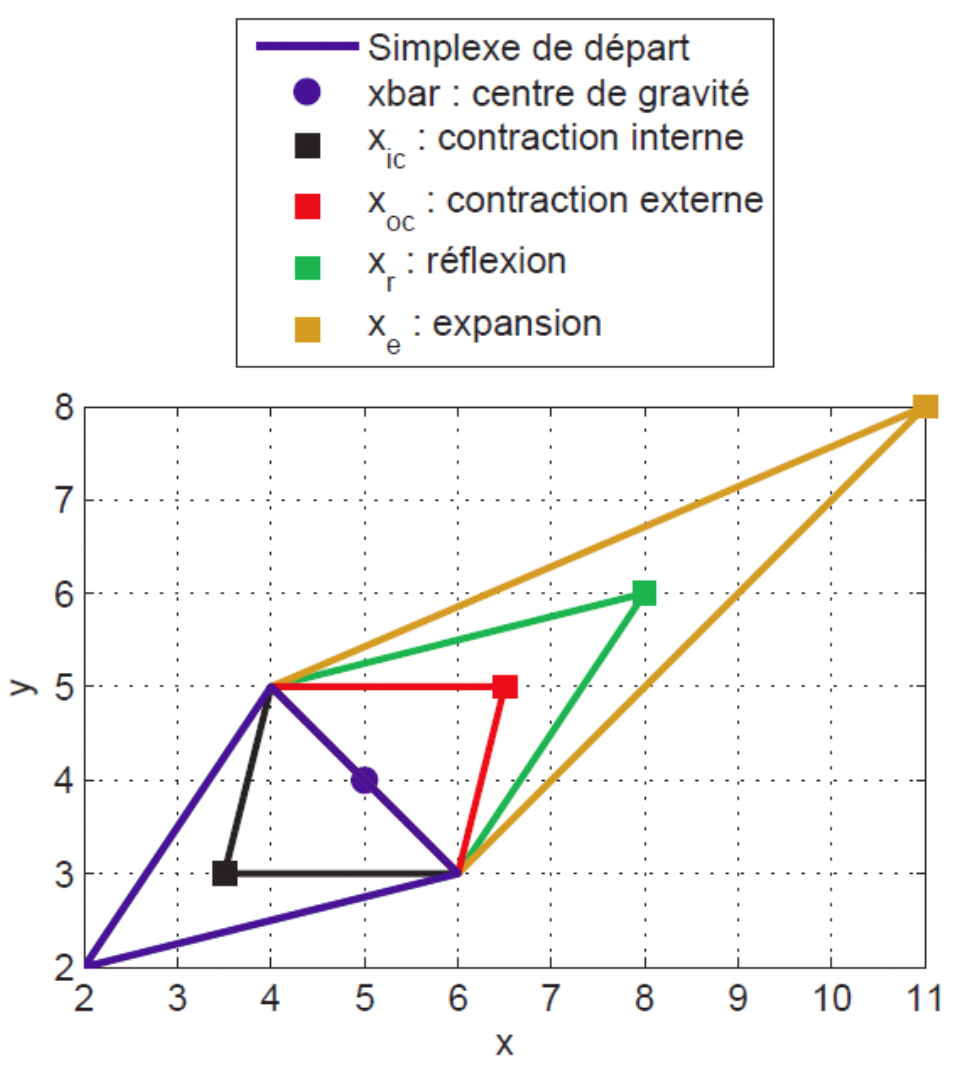
\includegraphics[width=0.3\textwidth]{neldermead.png}
     \caption*{Visualisation des étapes de la méthode du simplexe de Nelder-Mead.}
\end{figure}

\subsubsection{Résultats théoriques}

Les propriétés de la méthode sont assez faibles; il s'agit plus d'une heuristique
qui fonctionne bien en pratique.

On note par exemple que

\begin{itemize}
     \item pour une fonction strictement convexe à une variable, convergence vers le minimum global;
     \item pour une fonction strictement convexe à deux variables,
     convergence vers une valeur (pas nécessairement optimale) et donc il existe un simplexe
     $\Delta^{(0)}$ qui converge vers un point qui n'est pas un minimum d'une certaine fonction $f$.
\end{itemize}

\section{Aperçu d'optimisation avec contraintes}

On a le problème

\begin{equation*}
     \min_{x \in \Rn} f(x) \textnormal{ tel que } c_i(x) = 0 \textnormal{ pour } i \in \eqset \textnormal{ et } c_i(x) \geq 0 \textnormal{ pour } i \in \inset.
\end{equation*}

La plupart des méthodes sont basées sur la résolution
répétée de sous-problèmes sans contraintes.

Il y une myriade de méthodes pour cela.

\begin{itemize}
     \item \strong{Méthodes de pénalité}. On résout une série de problèmes non contraints
     dépendant d'un paramètre $\mu > 0$ de plus en plus petit.
     Par exemple, pour un problème avec uniquement des égalités :
     \begin{equation*}
          \min_{x \in \Rn} f(x) + \frac{1}{2\mu}\sum_{i \in \eqset} c_i^2(x).
     \end{equation*}
     \item \strong{Méthodes de pénalité exacte}. On résout un unique problème pour $\mu$ suffisament petit.
     Par exemple, pour un problème avec uniquement des égalités :
     \begin{equation*}
          \min_{x \in \Rn} f(x) + \frac{1}{2\mu} \sum_{i \in \eqset} \abs{c_i(x)}.
     \end{equation*}
     Par contre, cette fonction n'est pas différentiable.
     \item \strong{Méthode barrière}. On résout une série de problèmes non contraints dépendant d'un paramètre $\mu > 0$ de plus en plus petit.
     Par exemple, pour un problème avec uniquement des inégalités :
     \begin{equation*}
          \min_{x \in \Rn} f(x) - \mu \sum_{i \in \inset} \log(c_i(x)).
     \end{equation*}
     \item \strong{Techniques basées sur l'approximation locale}. On approxime autour de l'itéré courant par un problème de \emph{sequential quadratic programming}.
     \item \strong{Lagrangien augmenté}. On combine le Lagrangien avec une pénalité quadratique :
     \begin{equation*}
          \min \lagr_{\textnormal{A}}(x, \lambda, \mu) = f(x) - \sum_{i \in \eqset} \lambda_i c_i(x) + \frac{1}{2\mu} \sum_{j \in \eqset} c_j^2(x),
     \end{equation*}
     avec mises à jour successives de $\lambda$ et $\mu$.
     \item \strong{Astuces}. On peut aussi reformuler, substituer, etc\dots
\end{itemize}

%     _
%    / \   _ __  _ __   _____  _____
%   / _ \ | '_ \| '_ \ / _ \ \/ / _ \
%  / ___ \| | | | | | |  __/>  <  __/
% /_/   \_\_| |_|_| |_|\___/_/\_\___|

\annexe

\section{Exemples de problèmes d'optimisation linéaire}
\begin{myexem}[Problème diététique (ou du mélange)]
  Supposons qu'on ait différents aliments aux coûts $c_i$
  qui donnent chacun une certaine quantité de chaque élément $a_{ji}$ et
  qu'on ait besoin d'une quantité $b_j$ de chaque élément.
  \begin{center}
    \begin{tabular}{|l|c|c|c|c|c|}
      \hline
      & aliment 1 & aliment 2 & $\cdots$ & élément $n$ & contenu recherché\\
      \hline
      coûts & $c_1$ & $c_2$ & $\cdots$ & $c_n$ & \\
      \hline
      élément 1 & $a_{11}$ & $a_{12}$ & $\cdots$ & $a_{1n}$ & $b_1$\\
      \hline
      élément 2 & $a_{21}$ & $a_{22}$ & $\cdots$ & $a_{2n}$ & $b_2$\\
      \hline
      \multicolumn{1}{|c|}{$\vdots$} & $\vdots$ & $\vdots$
      & $\ddots$ & $\vdots$ & $\vdots$\\
      \hline
      élément $m$ & $a_{m1}$ & $a_{m2}$ & $\cdots$ & $a_{mn}$ & $b_m$\\
      \hline
    \end{tabular}
  \end{center}
  En posant $x_i$ comme la quantité qu'on prend de l'élément $i$,
  on sait modéliser le problème comme suit
  \begin{align*}
    \min \sum_i c_i x_i\\
    \sum_i a_{ji} x_i & = b_j\\
    x_i & \geq 0
  \end{align*}
  qui est un problème d'optimisation linéaire.
\end{myexem}

\begin{myexem}[Problème du transport]
  Soient $m$ sources de capacité $a_i$ et
  $n$ destinations de besoin $b_j$.
  Le transport d'une unité de $i$ à $j$ coûte $c_{ij}$.
  Posons $x_{ij}$ la quantité transportée de $i$ à $j$.
  On peut alors modéliser le problème par le problème d'optimisation linéaire
  suivant
  \begin{align*}
    \min \sum c_{ij} x_{ij}\\
    \sum_j x_{ij} & \leq a_i & \forall &i\\
    \sum_j x_{ij} & \geq b_i & \forall &i\\
    x_{ij} & \leq 0 & \forall &i,j
  \end{align*}

  L'ensemble des solutions admissibles est vide si
  $\sum_1^m a_i < \sum_1^n b_i$.
\end{myexem}

\section{Normes}
On peut définir différentes normes :
\begin{itemize}
  \item la norme $l^1$ définie par
    \[ \phantom{;} \norm{x}_1 \coloneqq \sum_i \abs{x_i}; \]
  \item la norme $l^2$ définie par
    \[ \phantom{;} \norm{x}_2 \coloneqq \sqrt{\sum_i x_i^2}; \]
  \item la norme $l^p$ définie par
    \[ \phantom{;} \norm{x}_p \coloneqq \left(\sum_i \abs{x_i}^p\right)^{1/p}; \]
  \item la norme $l^\infty$ définie par
    \[ \phantom{.} \norm{x}_\infty \coloneqq \max_i \abs{x_i}. \]
\end{itemize}

\section{Centre de Tchebychev}
\begin{mydef}[Centre de Tchebychev]
  Le centre de Tchebychev d'un polyèdre est le centre de la plus grande boule contenue dans ce polyèdre.
\end{mydef}
\begin{myrem}
  L'ensemble des centres de Tchebychev peut également être infini ou vide.
\end{myrem}
\begin{myprop}
  La distance entre un point $x_0$ et
  un hyperplan $H$ défini par $H\equiv a^Tx = b$ est
  \[ d(x_0, H) = \frac{\abs{b-a^Tx_0}}{\norm{a}}. \]
\end{myprop}

Soit un polyèdre $P = \{x\in\Rn \suchthat a_i^Tx \geq b_i\}$.
Supposons, sans perte de généralité, que $\norm{a_i} = 1$.
\begin{align*}
  d(x, P) & = \min_i \frac{\abs{a_i^Tx - b_i}}{\norm{a_i}}\\
  \max_{x\in P} d(x, P)
  & = \max_{x\in P}\min_i \abs{a_i^Tx - b_i}\\
  & = \max_{x\in P}\min_i a_i^Tx - b_i.\\
\end{align*}
On a donc
\begin{align*}
  \max_{x, t} t\\
  a_i^Tx - b_i & \geq t & \forall i\\
  x & \in P
\end{align*}
ou encore
\begin{align*}
  \max_{x, t} t\\
  a_i^Tx - t & \geq b_i & \forall i\\
  a_i^Tx & \geq b_i & \forall i. % useless car t >= 0 par def
\end{align*}
Si $z^* \geq 0$, $(\xopt, t^*)$ avec
$\xopt$, le centre de Tchebychev et $t^*$, le rayon.
$z^* < 0$ impossible par définition (on a viré les $|$).
On peut dire que $a_i^T\xopt -t^* \geq b_i$.

\section{Conjecture de Hirsch}
Soit un polyèdre borné $\polye$.
La distance entre deux sommets $x, y \in \polye$ d'un polyèdre
est définie par le plus petit nombre d'arêtes qu'on doit traverser pour aller
de $x$ à $y$.
Son diamètre $D(\polye) = \max_{x, y \in \polye} d(x, y)$.
$\Delta(n, m)$ est le diamètre maximal des polyèdres de $\Rn$
définis par $m$ inégalités.
La première version,
\[ \phantom{,} \Delta(n, m) \leq m-n, \]
a longtemps tenu mais est fausse comme le montre un contre-exemple trouvé
en 2010.
\[ \Delta(2, m) \leq \left\lfloor\frac{m}{2}\right\rfloor.\] % what use does this formula serve?
Heureusement, il existe une version faible (également postulée par Hirsch en 1957) :
\[ \phantom{,} \Delta(n, m) \leq P(n, m), \]
où $P$ est un polynôme.

\section{Preuves d'optimisation non linéaire}
\begin{mytheo}
  Si $\xopt$ est un min local de $\min_{x \in \Rn}f(x)$ alors
  $\gradn f(\xopt) = 0$.
  \begin{proof}
    Soit un point $x$ tel que $\gradn f(x) \neq 0$.
    On va montrer que $x$ n'est pas un min local.
    Soit $\Delta x  = -\theta \gradn f(x)$ pour un certain $\theta > 0$.
    On a
    \[ f(x + \Delta x) = f(x) - \theta\gradn f(x - \alpha\theta\Delta f(x))^T
    \Delta f(x). \]
    Considérons la fonction $g(t) = \gradn f(x - t\gradn f(x))^T \gradn f(x)$.
    \begin{enumerate}
      \item $g(0) > 0$ ($g(0) = \gradn f(x)^T\gradn f(x)
        = \norm{\gradn f(x)}^2 > 0$).
      \item $g$ est continue (car $\gradn f$ est continue).
    \end{enumerate}
    Par conséquent, $\exists t_\mathrm{max}$ tel que $g(t) > 0$
    $\forall t \suchthat 0 \leq t \leq t_\mathrm{max}$.
     On conclut que $f(x + \Delta x) < f(x)$ dès que
     $\theta \leq t_\mathrm{max}$.
  \end{proof}
\end{mytheo}

\begin{mytheo}[Bolzano-Weierstrass]
  Si $\{x_k\}_{k=1,\dots,\infty} \subseteq \mathcal{E}$ compact (fermé et borné), alors $\exists \{x_{u_k}\}$ où $u_1 < u_2 < \dots < u_k < \dots$
  (sous-suite) convergente vers un point de $\mathcal{E}$.
\end{mytheo}

\begin{myexem}
  $\min_{x \in \Rn} f(x)$.
  Considérons plutôt $\{f(x_k)\}_{k=1,\dots,\infty}$ sous l'hypothèse
  que $f(x_k) \leq f(x_0)$ et $f(x)$ bornée inférieurement.
  Alors il existe $u_1 < u_2 < \dots < u_k$ tels que $f(x_{u_k})$ converge.
  Si, de plus, $f(x_k) \leq f(x_{k-1})$ (monotonicité), la suite
  $f(x_k)$ converge.
  Attention, on n'a pas dit qu'on convergeait vers la valeur optimale.
\end{myexem}

\[ \alpha \mapsto x + \alpha p \mapsto \Phi(\alpha) \]
Donc $\Phi'(\alpha) = \grad f (x_k + \alpha p_k)^T p_k$.
$\Phi'(0) = \grad f (x_k)^Tp_k < 0$.
$\Phi(\alpha) \leq \Phi(0) + c_i\alpha\Phi'(0)$.

\begin{mytheo}[Théorème de Zoutendijk]

Posons :

\begin{equation}
     \label{H}
     f(x) \textnormal{ bornée inférieurement},
\end{equation}

\begin{equation}
     \label{desc}
     \grad f(x_k)^Tp_k < 0,
\end{equation}

\begin{equation}
     \label{w1}
     f(x_k + \alpha_kp_k) \leq f(x_k) + c_1\alpha_k \grad f(x_k)^Tp_k,
\end{equation}

\begin{equation}
     \label{w2}
     \grad f(x_k + \alpha_k p_k)^T p_k \geq c_2 (\grad f(x_k)^T p_k),
\end{equation}

\begin{equation}
     \label{lip}
     \norm{\grad f(y) - \grad f(x)} \leq L\norm{x - y}.
\end{equation}

  \begin{proof}
    Bornons la longueur $\alpha_k$ (par le bas) :
    \begin{align*}
      \grad f(x_k + \alpha_k p_k)^T p_k - \grad f(x_k)^T p_k &
      \geq (c_2 - 1) \grad f(x_k)^T p_k\\
      (\grad f(x_k + \alpha_kp_k) - \grad f(x_k))^T p_k &
      \geq (c_2 - 1) \grad f(x_k)^Tp_k > 0.
    \end{align*}

    Combinons avec \eqref{lip} :
    \[ \norm{\grad f(x_k + \alpha_kp_k) - \grad f(x_k)}
    \leq \alpha_k L \norm{p_k}. \]

    Par Cauchy-Schwartz :
    \[ (\grad f(x_k + \alpha_kp_k) - \grad f(x_k))^T p_k \leq
    \norm{\grad f(x_k + \alpha_kp_k - \grad f(x_k)} \norm{p_k}, \]

    d'où

    \[ \alpha_k \geq \frac{(c_2-1)\grad f(x_k)^Tp_k}{L\norm{p_k}^2}. \]

    Par \eqref{w1}, comme $c_1 \grad f (x_k)^T p_k$, on a
    \[ f(x_{k+1}) - f(x_k) \leq c_1 \frac{(c_2-1)}{L}
    \left(\frac{\grad f(x_k)^T p_k}{\norm{p_k}}\right)^2. \]

    En sommant de 0 à $k-1$, on obtient
    \[ f(x_k) - f(x_0) \leq \frac{c_1(c_2-1)}{L} \sum_{j = 0}^{k-1}
    \left(\frac{\grad f(x_j)^T p_j}{\norm{p_j}}\right)^2. \]

    Mais $f(\xopt) - f(x_0)$ est fini et
    $f(\xopt)-f(x_0) \leq f(x_k) - f(x_0)$.

    On conclut que
    \[ \sum_{k=0}^{+\infty} \frac{(\grad f(x_k)^T p_k)^2}{\norm{p_k}^2}
    \leq \frac{f(x_0) - f(\xopt)}{c_1(1-c_2)/L}. \]

    Puisque
    \[ -\grad f(x_k) p_k = \cos \theta_k \norm{\grad f(x_k)} \norm{p_k}, \]

    on a

    \[ \sum_{k=0}^{+\infty} \cos^2\theta_k \norm{\grad f(x_k)}^2 < \infty. \]
  \end{proof}
\end{mytheo}

\begin{mytheo}[Formule de la perturbation SR1]

\begin{proof}
La perturbation a la forme générale

\begin{equation*}
     B_{k+1} = B_k + \sigma v v^T,
\end{equation*}
où on a $\sigma = \rpm 1$ et $\sigma$ et $v$ sont choisis
pour que $B_{k+1}$ respecte la condition de la sécante (c'est-à-dire $y_k = B_{k+1} s_k$).

En substituant, on obtient

\begin{equation}
     \label{SR1plugin}
     y_k = B_k s_k + \left[\sigma v^T s_k\right] v.
\end{equation}

Le terme entre parenthèses doit être scalaire; on déduit donc que
$v$ est un multiple de $y_k - B_{k} s_k$, ou bien que
$v = \delta (y_k - B_{k} s_k)$ pour un certain scalaire $\delta$.
On remplace cette forme de $v$ dans \eqref{SR1plugin} pour obtenir

\begin{equation*}
     (y_k - B_{k} s_k) = \sigma \delta^2 \left[ s_k^T (y_k - B_{k} s_k) \right] (y_k - B_{k} s_k),
\end{equation*}

et il est clair que cette égalité est satisfaite
si et seulement si on choisit les paramètres $\delta$ et $\sigma$ suivants :

\begin{equation*}
     \sigma = \sign \left[ s_k^T (y_k - B_{k} s_k) \right], \qquad \delta = \rpm \abs{s_k^T (y_k - B_{k} s_k)}^{-1/2}.
\end{equation*}

Ainsi, on a montré que la seule perturbation symétrique de rang 1
qui satisfait la condition de la sécante est donnée par

\begin{equation*}
     B_{k+1} = B_k + \frac{(y_k - B_{k} s_k)(y_k - B_{k} s_k)^T}{(y_k - B_{k} s_k)^T s_k}.
\end{equation*}

Cette formule peut se transformer très facilement en

\begin{equation*}
     H_{k+1} = H_k + \frac{(s_k - H_{k} y_k)(s_k - H_{k} y_k)^T}{(s_k - H_{k} y_k)^T y_k}.
\end{equation*}

\end{proof}
\end{mytheo}

\end{document}
